\documentclass[12pt]{article}

\pagestyle{empty}
\setlength{\topmargin}{0in}
\setlength{\headheight}{0in}
\setlength{\topsep}{0in}
\setlength{\textheight}{9in}
\setlength{\oddsidemargin}{0in}
\setlength{\evensidemargin}{0in}
\setlength{\textwidth}{6.5in}

\usepackage{palatino, graphicx,amssymb}

\newcommand{\ds}{\displaystyle}
\newcommand{\vs}[1]{\vspace{#1in}}
\renewcommand{\vss}[1]{\vspace*{#1in}}
\newcommand{\bvec}{{\mathbf b}}
\newcommand{\cvec}{{\mathbf c}}
\newcommand{\dvec}{{\mathbf d}}
\newcommand{\evec}{{\mathbf e}}
\newcommand{\fvec}{{\mathbf f}}
\newcommand{\qvec}{{\mathbf q}}
\newcommand{\uvec}{{\mathbf u}}
\newcommand{\vvec}{{\mathbf v}}
\newcommand{\wvec}{{\mathbf w}}
\newcommand{\xvec}{{\mathbf x}}
\newcommand{\yvec}{{\mathbf y}}
\newcommand{\zvec}{{\mathbf y}}
\newcommand{\pvec}{{\mathbf p}}
\newcommand{\zerovec}{{\mathbf 0}}
\newcommand{\real}{{\mathbb R}}
\newcommand{\twovec}[2]{\left[\begin{array}{r}#1 \\ #2
    \end{array}\right]}
\newcommand{\ctwovec}[2]{\left[\begin{array}{c}#1 \\ #2
   \end{array}\right]}
\newcommand{\threevec}[3]{\left[\begin{array}{r}#1 \\ #2 \\ #3
  \end{array}\right]}
\newcommand{\cthreevec}[3]{\left[\begin{array}{c}#1 \\ #2 \\ #3
    \end{array}\right]}
\newcommand{\fourvec}[4]{\left[\begin{array}{r}#1 \\ #2 \\ #3 \\ #4
    \end{array}\right]}
\newcommand{\cfourvec}[4]{\left[\begin{array}{c}#1 \\ #2 \\ #3 \\ #4
    \end{array}\right]}
\newcommand{\fivevec}[5]{\left[\begin{array}{c}#1 \\ #2 \\ #3 \\ #4 \\
                                 #5 \\
    \end{array}\right]}
\newcommand{\mattwo}[4]{\left[\begin{array}{rr}#1 & #2 \\ #3 & #4 \\ \end{array}\right]}
\renewcommand{\span}[1]{\text{Span}\{#1\}}
\newcommand{\bcal}{{\cal B}}
\newcommand{\ccal}{{\cal C}}
\newcommand{\scal}{{\cal S}}
\newcommand{\wcal}{{\cal W}}
\newcommand{\ecal}{{\cal E}}
\newcommand{\coords}[2]{\left\{#1\right\}_{#2}}
\newcommand{\gray}[1]{\color{gray}{#1}}
\newcommand{\lgray}[1]{\color{lightgray}{#1}}
\newcommand{\rank}{\text{rank}}
\newcommand{\col}{\text{Col}}
\newcommand{\nul}{\text{Nul}}

\begin{document}

\noindent
{\bf Mathematics 227} \\ 
{\bf Lab 5, Due: December 7, 2018}

\bigskip
\noindent
{\bf Instructions:} The exercises here should be completed in groups
of 2 or 3 students with one write-up submitted from each group.

\medskip
So far, we have found eigenvalues by solving the characteristic
equation $\det(A-\lambda I) = 0$ and eigenvectors by solving the
homogeneous equation $(A-\lambda I)\xvec = \zerovec$.  In practice,
the matrices we'll be working with could be $10,000\times 10,000$ and
this approach is not practical:  finding the roots of
a $10,000$ degree polynomial is not practical and solving the homogeneous
equation is plagued by the fact that computers only perform
approximate arithmetic.  Forunately, there's a way to numerically find
eigenvectors using what's called the {\em power method}.

\begin{enumerate}
\item Let's look at the example
  $
  A =
  \left[
    \begin{array}{cc}
      0.5 & 0.2 \\
      0.4 & 0.7 \\
    \end{array}
  \right]
  $
  and the initial vector $\xvec_0=\twovec10$.

  Find the vector $\xvec_1 = A\xvec_0$.

  \vs{1}

  Then identify $m_1$, the component of $\xvec_1$ that has the largest
  absolute value, and form the new vector
  $
  \overline{\xvec}_1 = \frac{1}{m_1}\xvec_1$.  What is
  $\overline{\xvec}_1$?  Notice that the component of
  $\overline{\xvec}_1$ having the largest absolute value is 1.

  \vs{1}
  Repeat this process by finding $\xvec_2 = A\overline{\xvec}_1$.
  Then identify $m_2$, the component of $\xvec_2$ having the largest
  absolute value and form $\overline{\xvec}_2 =
  \frac{1}{m_2}\xvec_2$.

  \vs{1}
  This is clearly a process that can be automated.  There is a
  collection of Sage cells at the page
  {\tt http://gvsu.edu/s/0TD}.  The first cell there contains some
  useful commands so you should evaluate it now.

  \medskip
  In the second cell, define the matrix $A$ and vector $\xvec_0$ from
  above.  You can repeat the process we've outlined above by saying
  {\tt power(A, x0, 20)}.  When you do this, you will see the
  multiplier $m_j$ and the vectors $\overline{\xvec}_j$ appear.

  To what vector $\pvec$ does the sequence of vectors
  $\overline{\xvec}_j$ converge?  To what value do the multipliers
  $m_j$ converge?

  \vs{1}
  Find $A\pvec$ and verify that $\pvec$ is an eigenvector.  What is
  the corresponding eigenvalue?

  \vs{1}
  This technique is called the power method.  Explain how the power
  method computes the eigenvalue of $A$ having the largest absolute
  value and a corresponding eigenvector.

  \vs{1}
\item The power method finds the eigenvalue with the largest absolute
  value.  Suppose now that we want to find the eigenvalue with the
  smallest absolute value.  We can use the {\em inverse power method}
  to do this.

  If $\lambda$ is an eigenvalue of $A$ with eigenvector $\vvec$, then
  we know that 
  $$
  A\vvec = \lambda\vvec.
  $$
  If we multiply both sides by $\lambda^{-1}A^{-1}$, then we have
  $$
  A^{-1}\vvec = \lambda^{-1}\vvec.
  $$
  This means that $\lambda^{-1}$ is an eigenvalue of $A^{-1}$ with
  eigenvector $\vvec$.  
  Therefore, if $\lambda$ is the eigenvalue of $A$ having the smallest
  possible absolute value, then $\frac1{\lambda}$ is the eigenvalue of
  $A^{-1}$ having the largest possible absolute value.  This means
  that we can find $\frac{1}{\lambda}$, and hence $\lambda$, by
  applying the power method to $A^{-1}$.  This is called the 
  inverse power method.

  Back on the page of Sage cells, the command {\tt inverse\_power(A,
    x0, N)} applies the power method to $A^{-1}$.  Find the smallest
  eigenvalue of $A$ and a corresponding eigenvector.

  \vs{1}
\item Now define the matrix
  $$
  A = \left[
    \begin{array}{cccc}
      3.6 & 1.6 & 4.0 & 7.6 \\
      1.6 & 2.2 & 4.4 & 4.1 \\
      3.9 & 4.3 & 9.0 & 0.6 \\
      7.6 & 4.1 & 0.6 & 5.0 \\
    \end{array}
  \right].
  $$
  Use the power method and inverse power method to find the
  eigenvalues with the largest and smallest absolute values.

  \vs{1}

  Since $A$ is a $4\times4$ matrix, we expect that there should be two
  more eigenvalues.  How can we find them?

  Suppose that $s$ is some scalar.  Suppose also that $\vvec$ is
  an eigenvalue of $A$ with associated 
  eigenvalue $\lambda$.  Explain why $\vvec$ is also an eigenvector of
  $A-sI$.

  \vs{1}
  What is the eigenvalue of $A-sI$ associated to the eigenvector
  $\vvec$? 

  \vs{1}
  The eigenvalue of $A$ closest to $s$ is the eigenvalue
  of $A-sI$ closest to $0$, which is the eigenvalue of $A-sI$ having the
  smallest absolute value.  This means that we can find the eigenvalue
  of $A$ closest to some number $s$ by applying the inverse power
  method to $A-sI$.  You can find the eigenvalues of $A$ closest to
  some number $s$ by saying {\tt find\_closest\_eigenvalue(A, s, x0, 20)}.

  \newpage
  For the matrix $A$ above, you should have found the eigenvalues
  $\lambda_1 = 16.35$ and $\lambda_2 = 0.75$, which may be
  represented on a number line as shown.  The other eigenvalues must
  be in the gray shaded area.

  \begin{center}
    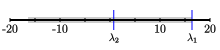
\includegraphics{numerical-power-line.eps}
  \end{center}

  Use the command {\tt find\_closest\_eigenvalue} to probe into the
  gray areas to find the other two eigenvalues.  What do you find?

  \vs{1}

\item The first Sage cell on that page defined the matrix
  $$
  B= \left[
    \begin{array}{rrrrr}
      -14.6 & 9.0 & -14.1 & 5.8 &  13.0 \\
      27.8 & -4.2 &  16.0 & 0.9 & -21.3 \\
      -5.5 & 3.4 &  3.4 &  3.3 &  1.1 \\
      -25.4 & 11.3 & -15.4 & 4.7 &  20.3 \\
      -33.7 & 14.8 & -22.5 & 9.7 &  26.6 \\
    \end{array}
  \right].
  $$

  Use the power method to find the eigenvalue with the largest
  absolute value, the eigenvalue with the smallest absolute value, and
  the other three eigenvalues.  You can keep track of your results on
  the number line below.  State your result by listing the eigenvalues
  in increasing order.

  \begin{center}
    \includegraphics{number-line.eps}
  \end{center}

  

  
  
    
  

  

\end{enumerate}






\end{document}